\chapter{Metodologia}
\label{chap:metodologia}

% ir na literatura e falar sobre o modelo que será utilizado. Fazer de forma macro, sem entrar em detalhe nas fórmulas. ## DESCREVER A IDEIA

% Usar RandomForest e NeuralNetwork

% 1. Ideia da Regressão linear 
% 2. Ideia do RandomForest (usar em pt-br: Floresta aleatória)
% 3. Ideia do NeuralNetwork. (explicar só a de regressão) Vamos utilizar uma rede para regressão

O primeiro passo, que possibilitou o desenvolvimento do trabalho como um todo, foi o recebimento dos dados do processamento de cimento, na fábrica Apodi. \textbf{(... falar sobre os dados. Estrutura, colunas, etc...) (Falar sobre possíveis tratativas que foram necessárias ser feitas)}. Após a realização da curagem dos dados, pudemos partir para uma análise mais aprofundada, a fim de entender com o que estávamos trabalhando, através de uma análise exploratória dos dados. \textbf{(Falar sobre técnicas utilizadas na EDA... Mediana, média, boxplot, correlação, desvio padrão, etc...)}

Com o entendimento solidificado acerca do conjunto de dados, o próximo passo foi a aplicação dos modelos empregados que serão responsáveis pela predição do comportamento vibratório dos moinhos de rolos verticais.

\section{Inteligência artificial}

A inteligência artificial (IA) trata-se do campo que se concentra na pesquisa e no avanço de algoritmos que podem compreender e exibir comportamento inteligente, sem a intervenção humana no entendimento ou sem explicitamente dizer como responder a determinados estímulos \cite{Dinesh2024}. Os modelos de IA podem ser vistos nos smartphones, nos carros, nos bancos, nos hospitais, na aplicação da lei, nas organizações de seguros e em muitas outras aplicações \cite{Ali2023}.
 
\section{Regressão linear}

Nesse trabalho, a base geral de método preditivo aplicado foi a regressão linear. A qual, de acordo com \cite{HESAMIAN2024}, ajuda a identificar e quantificar as relações entre as variáveis, permitindo previsões e compreensão do impacto das variáveis independentes na variável dependente. 

Segundo \cite{Schneider2010}, a regressão linear é utilizada para estudar a relação linear entre uma variável dependente Y e uma ou mais variáveis independentes X. A variável dependente Y deve ser contínua, enquanto as variáveis independentes podem ser contínuas, binárias ou categóricas. O julgamento inicial de uma possível relação entre duas variáveis contínuas deve sempre ser feito com base em um gráfico de dispersão. Este tipo de gráfico mostrará se a relação é linear (figura \ref{fig:relacao-linear}) ou não linear (figura \ref{fig:relacao-exponencial}).

\pagebreak

 	\begin{figure}[h!] 
   	    \captionsetup{width=6cm}%Da mesma largura que a figura
		\Caption{\label{fig:relacao-linear} Gráfico de dispersão com relação linear.}
		\UFCfig{}{
			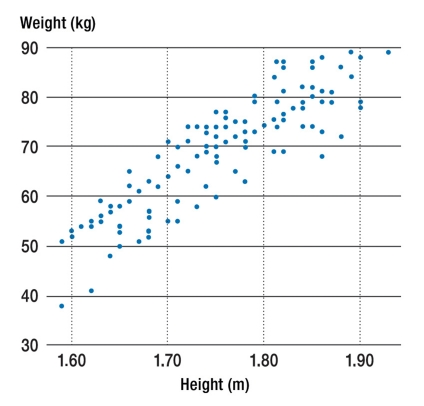
\includegraphics[width=6cm]{figuras/A scatter plot showing a linear relationship.jpg}
		}{
			\Fonte{\cite{Schneider2010}.}
		}	
	\end{figure}

  	\begin{figure}[h!] 
   	    \captionsetup{width=6cm}%Da mesma largura que a figura
		\Caption{\label{fig:relacao-exponencial} Gráfico de dispersão com relação exponencial.}
		\UFCfig{}{
			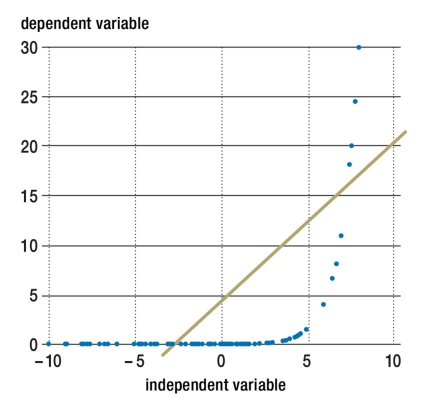
\includegraphics[width=6cm]{figuras/A scatter plot showing an exponential relationship.jpg}
		}{
			\Fonte{\cite{Schneider2010}.}
		}	
	\end{figure}

Quando temos uma relação linear, podemos dizer que as variáveis são correlacionadas em determinados graus. Porém, correlação não implica causalidade, e deve-se tomar cuidado para não tomar esse único indício como definitivo.

\pagebreak


\section{Floresta aleatória}

Falando de modelos de aprendizado de máquina, o primeiro utilizado baseia-se no princípio da floresta aleatória, a qual, de acordo com \cite{Wang2023}, é um método de aprendizado em conjunto que combina múltiplas árvores de decisão, usando \textit{bagging} (amostragem \textit{Bootstrap}) para reamostrar os dados originais e construir novos conjuntos de treinamento. Cada conjunto é usado para construir uma árvore de decisão, e a previsão final é feita pela média das saídas dessas árvores. Floresta aleatória é conhecida por sua escalabilidade e capacidade de lidar com dados de alta dimensão com menos parâmetros de otimização em comparação com outros métodos como Redes Neurais de Retropropagação (BPNN) e Regressão de Vetores de Suporte (SVR). Um esquema representativo de uma floresta aleatória é mostrado na figura \ref{fig:esquema-floresta-aleatoria}.

  	\begin{figure}[h!] 
   	    \captionsetup{width=12cm}%Da mesma largura que a figura
		\Caption{\label{fig:esquema-floresta-aleatoria} Esquema representativo de uma floresta aleatória.}
		\UFCfig{}{
			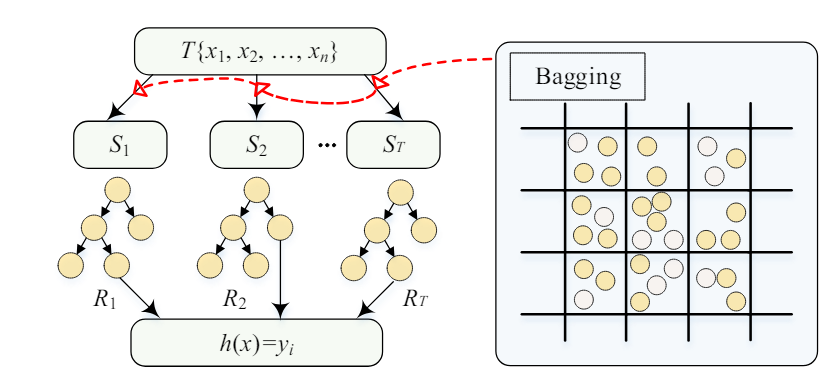
\includegraphics[width=12cm]{figuras/esquema-floresta-aleatoria.png}
		}{
			\Fonte{\cite{Wang2023}.}
		}	
	\end{figure}

 \subsection{Etapas de Implementação de uma floresta aleatória}

Primeiramente, a amostragem \textit{Bootstrap} é utilizada para reamostrar os dados originais, criando $T$ conjuntos de treinamento rotulados $S_1, S_2, \ldots, S_T$. Esses conjuntos de treinamento são então utilizados para construir árvores de regressão correspondentes $R_1, R_2, \ldots, R_T$. A cada nó, são amostrados aleatoriamente $T$ atributos de $M$, e o método de divisão ótima é aplicado utilizando o algoritmo CART, construindo o modelo $y = h(x)$. Para amostras de teste desconhecidas, calculam-se os valores previstos $R_1(X), R_2(X), \ldots, R_T(X)$ de cada árvore, e a média desses valores é usada como previsão final \cite{Wang2023}.

Devido à amostragem \textit{Bootstrap}, nem todos os dados originais são incluídos nos novos conjuntos de treinamento. Os dados excluídos formam a amostra \textit{Out-of-Bag (OOB)}, que é utilizada para validação cruzada embutida, avaliando o desempenho das árvores e estimando erros de generalização não tendenciosos \cite{Wang2023}.

 \subsection{Hiperparâmetros}

Os principais hiperparâmetros a serem ajustados são a profundidade das árvores e o número de preditores amostrados em cada nó. Árvores profundas tendem a \textit{overfitting}, enquanto árvores rasas podem sofrer de \textit{underfitting}. O número de preditores amostrados em cada nó afeta a precisão da previsão e precisa ser ajustado cuidadosamente para alcançar o melhor modelo \cite{Wang2023}.



\section{Redes neurais}

Segundo \cite{Kufel2023}, redes neurais artificiais se assemelham ao cérebro humano (Figura \ref{fig:diagrama-simplificado-neuoronio-humano}) e são compostas por múltiplos perceptrons ou ‘neurônios’ que processam e transmitem informações. Para entender seu funcionamento (Figura \ref{fig:esquema-nn}), começamos com a entrada de dados, como imagens, textos ou sons. Esses dados percorrem a rede, sendo processados por camadas sucessivas de neurônios até chegar à saída. Cada camada contém múltiplos neurônios que processam os dados de entrada.

\pagebreak

   	\begin{figure}[h!] 
   	    \captionsetup{width=12cm}%Da mesma largura que a figura
		\Caption{\label{fig:diagrama-simplificado-neuoronio-humano} Diagrama simplificado de um neurônio humano. 1—dendritos, local de entrada de sinal, 2—núcleo do neurônio, 3—zona de iniciação (onde o potencial de ação do neurônio é formado), 4—axônio, e 5—terminações axonais (que formam conexões com outras células e são os locais de saída de sinal), respectivamente.}
		\UFCfig{}{
			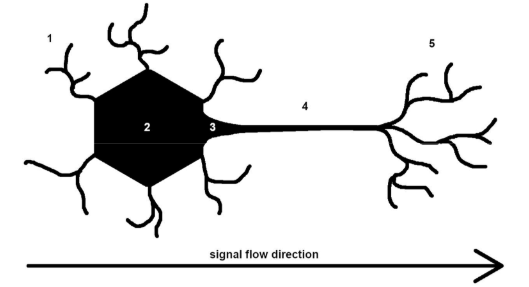
\includegraphics[width=12cm]{figuras/diagrama-simplificado-neuronio-humano.png}
		}{
			\Fonte{\cite{Kufel2023}.}
		}	
	\end{figure}

  	\begin{figure}[h!] 
   	    \captionsetup{width=12cm}%Da mesma largura que a figura
		\Caption{\label{fig:esquema-nn} Diagrama simplificado de um neurônio matemático. 1—entradas de sinal, 2—pesos, 3—somador, 4—ativador (função de ativação), e 5—saída de sinal, respectivamente.}
		\UFCfig{}{
			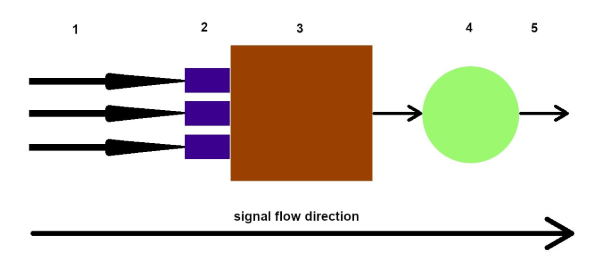
\includegraphics[width=12cm]{figuras/esquema-nn.png}
		}{
			\Fonte{\cite{Kufel2023}.}
		}	
	\end{figure}


 \pagebreak

Para treinar os perceptrons, os pesos são ajustados para minimizar a diferença entre a saída e o sinal esperado. A rede também aprende através do método da maior queda do gradiente, ajustando os comprimentos dos passos na direção oposta. Se o valor alvo em um novo ponto superar o ponto de partida, os passos são reduzidos até que o valor desejado seja alcançado (Figura \ref{fig:diagrama-nn}).

  	\begin{figure}[h!] 
   	    \captionsetup{width=10cm}%Da mesma largura que a figura
		\Caption{\label{fig:diagrama-nn} Diagrama simplificado da operação de uma rede neural.}
		\UFCfig{}{
			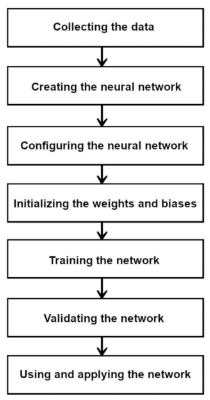
\includegraphics[width=10cm]{figuras/diagrama-nn.png}
		}{
			\Fonte{\cite{Kufel2023}.}
		}	
	\end{figure}

 \section{Long Short Term Memory (LSTM) Neural Network}

O modelo \textit{Long Short Term Memory (LSTM)} é uma evolução das Redes Neurais Recorrentes (RNN), que são compostas de várias camadas ocultas de neurônios em sequência, entre a camada de entrada e saída. O LSTM surgiu com o objetivo de resolver problemas típicos de RNN, como a perda de informações ao longo das camadas. As LSTMs são um tipo especial de RNN, capazes de aprender dependências de longo prazo e lembrar informações por períodos prolongados de tempo. A estrutura geral da LSTM também é de cadeia. Porém, em vez de uma única rede neural, existem quatro camadas com um método único de comunicação entre elas. A estrutura geral de uma LSTM pode ser observada na Figura \ref{fig:structure-of-a-lstm}.

  	\begin{figure}[h!] 
   	    \captionsetup{width=12cm}%Da mesma largura que a figura
		\Caption{\label{fig:structure-of-a-lstm} Estrutura de uma rede neural LSTM.}
		\UFCfig{}{
			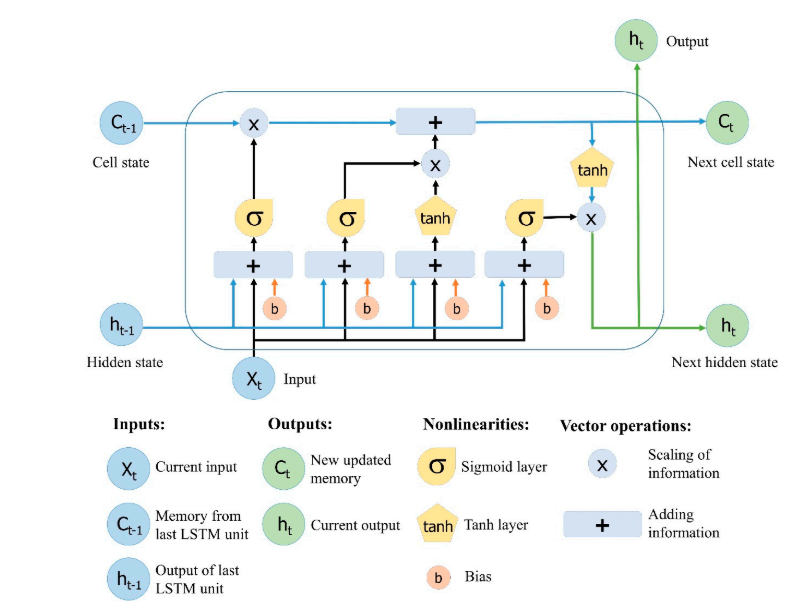
\includegraphics[width=12cm]{figuras/structure-of-a-lstm.png}
		}{
			\Fonte{\cite{Yan2016}.}
		}	
	\end{figure}

 % usar diagrama próprio

 começar pela exploração de dados
- separar variáveis que serão utilizadas, aquelas que acho que influenciam
- plotar gráficos de séries temporais de cada uma. Identificar ruídos e como removê-los

fazendo e escrevendo...
 

\section{Exemplo de alíneas}\label{sec:exemplo-de-algoritmos-e-figuras}

    Texto texto texto texto texto texto texto texto texto texto texto texto texto texto texto texto texto texto texto texto texto texto texto texto texto texto texto texto texto texto texto texto texto texto texto texto texto texto texto texto texto texto texto texto texto texto texto texto texto texto texto texto texto texto texto texto texto texto texto texto texto texto texto texto texto texto texto texto texto.

    %\begin{algorithm}[h!]
    %	\SetSpacedAlgorithm
    %	\caption{\label{exemplo-de-algoritmo}Como escrever algoritmos no \LaTeX2e}
    %	\Entrada{o proprio texto}
    %	\Saida{como escrever algoritmos com  Latex:}% \LaTeX2e }
    %	\Inicio{
    %		inicialização;
    %		\Repita{fim do texto}{
    %			leia o atual;
    %			\Se{entendeu}{
    %				vá para o proximo\;
    %				próximo se torna o atual;}
    %			\Senao{volte ao início da seção;}
    %		}
    %	}	
    %\end{algorithm}

    Texto texto texto texto texto texto texto texto texto texto texto.

    %\begin{algorithm}[H]
    %	\Entrada{o proprio texto}
    %	\Saida{como escrever algoritmos com \LaTeX2e }
    %	\Inicio{
    %		inicialização\;
    %		\Repita{fim do texto}{
    %			leia o atual\;
    %			\Se{entendeu}{
    %				vá para o próximo\;
    %				próximo se torna o atual\;}
    %			\Senao{volte ao início da seção\;}
    %		}
    %	}
    %	\caption{Exemplo de Algoritmo Versao 02}
    %\end{algorithm}

    %\begin{algorithm}
    %	\begin{algorithmic}
    %	\Entrada{o proprio texto}
    %	\Saida{como escrever algoritmos com \LaTeX2e }	
    %	\end{algorithmic}
    %\end{algorithm}

    Exemplo de alíneas com números:

    \begin{alineascomnumero}
	    \item Texto texto texto texto texto texto texto texto texto texto texto texto .
	    \item Texto texto texto texto texto texto texto texto texto texto texto texto .
	    \item Texto texto texto texto texto texto texto texto texto texto texto texto .
	    \item Texto texto texto texto texto texto texto texto texto texto texto texto .
	    \item Texto texto texto texto texto texto texto texto texto texto texto texto .
	    \item Texto texto texto texto texto texto texto texto texto texto texto texto .
    \end{alineascomnumero}

    Texto texto texto texto texto texto texto texto texto texto texto texto texto texto texto texto texto texto texto texto texto texto texto texto texto texto texto texto texto texto texto texto texto texto texto texto texto texto texto texto texto texto texto texto texto texto texto texto texto texto texto texto texto texto texto texto texto texto texto texto texto texto texto texto texto texto texto texto texto.

    Ou então figuras podem ser incorporadas de arquivos externos, como é o caso da \autoref{fig-grafico-1}. Se a figura que ser incluída se tratar de um diagrama, um gráfico ou uma ilustração que você mesmo produza, priorize o uso de imagens vetoriais no formato PDF. Com isso, o tamanho do arquivo final do trabalho será menor, e as imagens terão uma apresentação melhor, principalmente quando impressas, uma vez que imagens vetorias são perfeitamente escaláveis para qualquer dimensão. Nesse caso, se for utilizar o Microsoft Excel para produzir gráficos, ou o Microsoft Word para produzir ilustrações, exporte-os como PDF e os incorpore ao documento conforme o exemplo abaixo. No entanto, para manter a coerência no uso de software livre (já que você está usando LaTeX e abnTeX),  teste a ferramenta InkScape\index{InkScape}. ao CorelDraw\index{CorelDraw} ou ao Adobe Illustrator\index{Adobe! Illustrator}.  De todo modo, caso não seja possível  utilizar arquivos de imagens como PDF, utilize qualquer outro formato, como JPEG, GIF, BMP, etc.  Nesse caso, você pode tentar aprimorar as imagens incorporadas com o software livre \index{Gimp}Gimp. Ele é uma alternativa livre ao Adobe Photoshop\index{Adobe! Photoshop}.

\section{Usando fórmulas matemáticas}

Para escrever um símbolo matemático no texto, escreva símbolo entre cifrões, por exemplo, $\alpha$, $\beta$ e $\gamma$ são símbolo do alfabeto grego. Se você quiser inserir equações enumeradas, siga a estrutura de
\begin{equation}
    \label{eq:indices}
	k_{n+1} = n^2 + k_n^2 - k_{n-1}.
\end{equation}
Observe a pontuação, pois a equação faz parte da frase e do parágrafo. Como a equação faz parte da frase, não se utiliza o \textit{label} numérico \ref{eq:indices}. 

Quando for citar a Equação \ref{eq:indices} novamente no texto, utiliza-se o \textit{label} numérico. Repare que a palavra ``Equação'' foi escrita com ``E'' maiúsculo. 

Um exemplo de equações com frações é dado por
\begin{equation}
	\label{eq:fracao}
		\begin{aligned}
			x = a_0 + \cfrac{1}{a_1
				+ \cfrac{1}{a_2
					+ \cfrac{1}{a_3 + \cfrac{1}{a_4} } } }.
		\end{aligned}
	\end{equation}

Texto texto texto texto texto texto texto texto texto texto texto texto texto texto texto texto texto texto texto texto texto texto texto texto texto texto texto texto texto texto texto texto texto texto texto texto texto texto texto texto texto texto texto texto texto texto texto texto texto texto texto texto texto texto texto texto texto texto texto texto texto texto texto texto texto texto texto texto texto
	\begin{equation}
		\begin{aligned}
			k_{n+1} = n^2 + k_n^2 - k_{n-1}.
		\end{aligned}
	\end{equation}
	
Texto texto texto texto texto texto texto texto texto texto texto texto texto texto texto texto texto texto texto texto texto texto texto texto texto texto texto texto texto texto texto texto texto texto texto texto texto texto texto texto texto texto texto texto texto texto texto texto texto texto texto texto texto texto texto texto texto texto texto texto texto texto texto texto texto texto texto texto texto
	\begin{equation}
	\label{eq:trigo}
		\begin{aligned}
			\cos (2\theta) = \cos^2 \theta - \sin^2 \theta
		\end{aligned}.
	\end{equation}
	
Texto texto texto texto texto texto texto texto texto texto texto texto texto texto texto texto texto texto texto texto texto texto texto texto texto texto texto texto texto texto texto texto texto texto texto texto texto texto texto texto texto texto texto texto texto texto texto texto texto texto texto texto texto texto texto texto texto texto texto texto texto texto texto texto texto texto texto texto texto
	\begin{equation}
	\label{eq:matriz}
		\begin{aligned}
			A_{m,n} =
			\begin{pmatrix}
			a_{1,1} & a_{1,2} & \cdots & a_{1,n} \\
			a_{2,1} & a_{2,2} & \cdots & a_{2,n} \\
			\vdots  & \vdots  & \ddots & \vdots  \\
			a_{m,1} & a_{m,2} & \cdots & a_{m,n}
			\end{pmatrix}
		\end{aligned}.
	\end{equation}

Texto texto texto texto texto texto texto texto texto texto texto texto texto texto texto texto texto texto texto texto texto texto texto texto texto texto texto texto texto texto texto texto texto texto texto texto texto texto texto texto texto texto texto texto texto texto texto texto texto texto texto texto texto texto texto texto texto texto texto texto texto texto texto texto texto texto texto texto texto
	\begin{equation}
	\label{eq:sistema}
		\begin{aligned}
			f(n) = \left\{ 
			\begin{array}{l l}
			n/2 & \quad \text{if $n$ is even}\\
			-(n+1)/2 & \quad \text{if $n$ is odd}
			\end{array} \right.
		\end{aligned}.
	\end{equation}
Texto texto texto texto texto texto texto texto texto texto texto texto texto texto texto texto texto texto texto texto texto texto texto texto texto texto texto texto texto texto texto texto texto texto texto texto texto texto texto texto texto texto texto texto texto texto texto texto texto texto texto texto texto texto texto texto texto texto texto texto texto texto texto texto texto texto texto texto texto

%\section{Usando Algoritmos}

%\begin{algorithm}[h!]
%	\SetSpacedAlgorithm
%	\caption{\label{alg:algoritmo_de_colonica_de_formigas}Algoritmo de Otimização por Colônia de Formiga}
%	\Entrada{Entrada do Algoritmo}
%	\Saida{Saida do Algoritmo}
%	\Inicio{
%		Atribua os valores dos parâmetros\;
%		Inicialize as trilhas de feromônios\;
%		\Enqto{não atingir o critério de parada}{
%			\Para{cada formiga}{
%				Construa as Soluções\;
%			}
%			Aplique Busca Local (Opcional)\;
%			Atualize o Feromônio\;
%		}	
%	}		
%\end{algorithm}

\section{Usando código-fonte}

Um exemplo de código-fonte, ou código de programação encontra-se no Apendice \ref{ap:A}.

 
\section{Usando teoremas, proposições, etc}

 Texto texto texto texto texto texto texto texto texto texto texto texto texto texto texto texto texto texto texto texto texto texto texto texto texto.

\begin{teo}[Pitágoras]
	Em todo triângulo retângulo o quadrado do comprimento da
	hipotenusa é igual a soma dos quadrados dos comprimentos dos catetos. Usando o Apêndice \ref{ap:C}
\end{teo}


Texto texto texto texto texto texto texto texto texto texto texto texto texto texto texto.

\begin{teo}[Fermat]
	Não existem inteiros $n > 2$, e $x, y, z$ tais que $x^n + y^n = z$
\end{teo}

Texto texto texto texto texto texto texto texto texto texto texto texto texto texto texto.

\begin{prop}
	Para demonstrar o Teorema de Pitágoras...
\end{prop}

Texto texto texto texto texto texto texto texto texto texto texto texto texto texto texto.

\begin{exem}
	Este é um exemplo do uso do ambiente exem definido acima.
\end{exem}

Texto texto texto texto texto texto texto texto texto texto texto texto texto texto texto.


\begin{xdefinicao}
	Definimos o produto de ...
\end{xdefinicao}

Texto texto texto texto texto texto texto texto texto texto texto texto texto texto texto.

\section{Usando Questões} 

Um exemplo de questionário encontra-se no Apêndice \ref{ap:B}.

%Movido para o Apêndice

